\chapter{绪论}\label{cha:intro}
本章首先阐述论文的选题背景和意义(\ref{sec:background}节);随后介绍与工作流网相关的预备知识(\ref{sec:preliminaries}节);\ref{sec:challenge}重点讨论当前算法所面临的挑战;\ref{sec:contribution}节给出论文的主要贡献;最后\ref{sec:structure}节介绍论文的章节安排。

\section{选题背景和意义}\label{sec:background}
如今信息系统需要支持业务过程的执行,而不是像以往一样仅仅关注于独立的任务。信息系统需要控制、监控并且支持一个业务过程逻辑层面的全部内容,即它应该能管理组织内的工作流。很多拥有大量业务过程的组织和企业对工作流的管理有着极为迫切的需求,这正是工作流管理兴起的原因\cite{van1998application}。在工作流管理技术的帮助下,企业可以快速建立或者更新自身的过程感知信息系统\cite{dumas2005process}。企业可以根据市场变化或者政府政策变更等外部因素随时调整自己的业务过程从而及时地改善自身的服务以提高企业的市场竞争力。

过程感知信息系统是由实际业务过程模型驱动的,这些模型描述了企业中的业务执行过程,每个任务的负责人以及需要的资源和产生的数据等。由于同一个业务过程可以被不同拓扑结构的图形所表示,因此它的行为语义才是刻画该过程的本质特征。任务间有序关系\cite{esparza2002improvement}常常被用来描述业务过程的行为。业务过程的任务间有三种基本的有序关系:因果关系(causal relation)描述一个任务的完成导致了另一个任务被执行,并行关系(concurrency relation)表示两个任务可以同时执行互不影响,冲突关系(conflict relation)表示在业务过程的同一个执行实例中两个任务不能都被执行。

两个有因果关系或者并行关系的任务可能在同一个过程执行实例中出现,但是在部分执行实例中一个任务被执行,另一个任务的执行却不是必然的。因此,本文对这两种有序关系进行精炼以体现这种不确定性。处于冲突关系的两个任务显然不能在同一个执行实例中出现,所以没有必要对冲突关系进行精炼。

\begin{figure}[htbp]
  \centering
  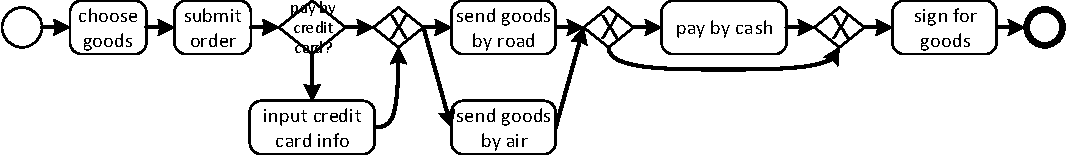
\includegraphics[width=1.0\textwidth]{basic_causal_drawback}
  \caption{含有不同因果关系的在线购物BPMN模型\label{fig:basic_causal_drawback}}
\end{figure}

\begin{example}\label{ex:basic_causal_drawback}
图\ref{fig:basic_causal_drawback}展示了一个在线购物的BPMN模型\footnote{BPMN是一种工作流建模语言,请参见:http://www.bpmn.org/}。在这个模型中,当任务“choose goods”被执行后,任务“submit order”可以被执行,然后任务“send goods by road”和任务“send goods by air”的其中之一可以被执行。显然,任务“choose goods”和任务“submit order”、任务“submit order”和任务“send goods by road”都满足因果关系。然而,这两组因果关系是不完全相同的。当任务“choose goods”被执行后,任务“submit order”一定会被执行而当任务“submit order”被执行后,任务“send goods by road”却不一定会被执行(因为任务“send goods by air”可能被选择执行)。前文提到的基本因果关系不能表达这类不同,所以需要对因果关系进行精炼。
\end{example}

\begin{figure}[htbp]
  \centering
  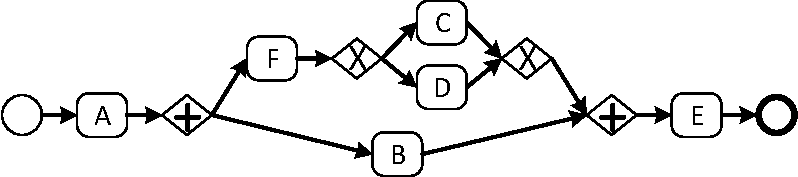
\includegraphics[width=1.0\textwidth]{basic_concurrency_drawback}
  \caption{含有不同并行关系的BPMN模型\label{fig:basic_concurrency_drawback}}
\end{figure}

\begin{example}\label{ex:basic_concurrency_drawback}
图\ref{fig:basic_concurrency_drawback}展示了一个含有并行结构的BPMN模型。在这个模型中,任务“B”和任务“C”可以被并行地执行但当任务“B”被执行时,任务“C”不一定会在同一个执行实例中被执行(因为任务“D”可能被选择执行)。同时,任务“B”和任务“F”也可以被并行地执行而且当任务“B”被执行时,任务“F”一定会在同一个执行实例中被执行。前文提到的基本并行关系不能表达这类不同,所以需要对并行关系进行精炼。
\end{example}

过程模型的任务间不确定性精炼有序关系(以下简称“精炼有序关系”)可以用来刻画过程的行为语义,从而被用于过程模型的检索,即提供一个查询模型$M$和一个过程模型集合$C$,从$C$中查找和$M$行为一致或者最相似的模型。由于本文的方法对过程模型进行了唯一的刻画,所以在检索过程中可以设置不同的粒度以检索符合实际要求的模型。除此之外,精炼有序关系还可以应用于过程模型的符合性检测、相似性度量等领域。

\begin{figure}[htbp]
  \centering
  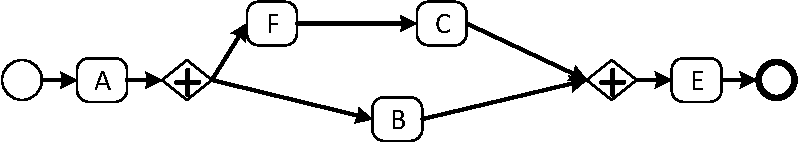
\includegraphics[width=1.0\textwidth]{basic_concurrency_drawback_compare}
  \caption{由图\ref{fig:basic_concurrency_drawback}改造得到的BPMN模型\label{fig:basic_concurrency_drawback_compare}}
\end{figure}

\begin{example}\label{ex:basic_concurrency_drawback_compare}
考虑图\ref{fig:basic_concurrency_drawback}和图\ref{fig:basic_concurrency_drawback_compare}中的模型,当检索满足条件“任务`F'和任务`C'满足因果关系且任务`B'和任务`C'满足并行关系”的模型时,两个模型都符合检索条件。另一方面,将检索条件更改为“任务`F'和任务`C'满足因果关系,且当任务`F'被执行时,任务`C'一定在同一个执行实例中被执行,同时当任务`C'被执行时,任务`F'一定在同一个执行实例中被执行;任务`B'和任务`C'满足并行关系,当任务`B'被执行时,任务`C'一定在同一个执行实例中被执行,同时当任务`C'被执行时,任务`B'一定在同一个执行实例中被执行”时,只有图\ref{fig:basic_concurrency_drawback_compare}中的模型符合条件。显然,精炼后的任务间有序关系能够更加精确地刻画过程模型的行为语义。类似的,这种精炼后的刻画方法可以被当作业务规则用于过程模型的符合性检测。
\end{example}

Jin等人已经提出了一种精炼有序关系RORU及其计算方法\cite{jin2014computing},本文重点对其进行了研究。针对该方法存在的问题,本文提出了改进方案,将新的方法命名为扩展的任务间不确定性精炼有序关系(Extended Refined Ordering Relations with Uncertainty,简称ExRORU)。由于ExRORU是一种刻画过程行为语义的方法,因此在实验过程中,本文将ExRORU与基于行为语义的过程特征刻画算法和过程相似性度量算法进行比较。

\section{预备知识}\label{sec:preliminaries}
本节介绍论文中需要用到的预备知识,其中\ref{subsec:petrinet}介绍Petri网,\ref{subsec:workflow_net}介绍工作流网及相关概念,\ref{subsec:process_run}和\ref{subsec:cpu}分别介绍过程流和完全前缀展开。

\subsection{Petri网}\label{subsec:petrinet}
业务过程建模给业务过程分析人员提供了建立过程模型并分析它们的能力,有许多论著和建模工具对其进行详尽地描述和实现。建模语言是业务过程建模中的核心部分,目前的建模语言包括但不限于:Petri网、EPC(Event-driven process chain,事件驱动过程链)、BPMN(Business Process Model and Notation,业务过程建模符号)、BPEL(Business Process Execution Language,业务过程执行语言)、UML(Unified Modeling Language,统一建模语言)、APROMORE\cite{la2011apromore}。

Petri网是一种有向二分图,于1960年代由Carl Adam Petri发明\cite{petri1962kommunikation},适合于描述含有异步、并发过程的系统。Petri网既有严格的数学表述方式,也有良好的图形化基础。本文使用Petri网作为建模语言,以下概念来自\onlinecite{van2004workflow}。有关Petri网及其性质的详细介绍,请参见\onlinecite{desel2005free,murata1989petri,reisig1998lectures,袁祟义2005petri}。

\begin{definition}[Petri网]\label{def:petrinet}
Petri网是一个三元组$N=(P,T,F)$,其中:
  \begin{itemize}
  	\item[-] $P$是库所的有限集合;
  	\item[-] $T$是变迁的有限集合;
  	\item[-] $P\cap T=\emptyset$且$T\cap P=\emptyset$;
  	\item[-] $F\subseteq(P\times T)\cup(T\times P)$是边的集合。
  \end{itemize}
\end{definition}

\begin{definition}[标识Petri网]\label{def:marked_petrinet}
标识Petri网是一个二元组$(N,s)$,其中$N=(P,T,F)$是一个Petri网,$s:P\rightarrow\mathbb{N}$是一个函数,表示网的标识。所有标识Petri网的集合记作$\mathcal{N}$。
\end{definition}

令$N=(P,T,F)$是一个Petri网。$P\cup T$中的元素称作节点。节点$x$是节点$y$的输入节点,当且仅当$(x,y)\in F$;节点$x$是节点$y$的输出节点,当且仅当$(y,x)\in F$。对于任意节点$x\in P\cup T$,$x$的前集$\bullet x=\{y|(y,x)\in F\}$,$x$的后集$x\bullet=\{y|(x,y)\in F\}$。

\begin{figure}[htbp]
  \centering
  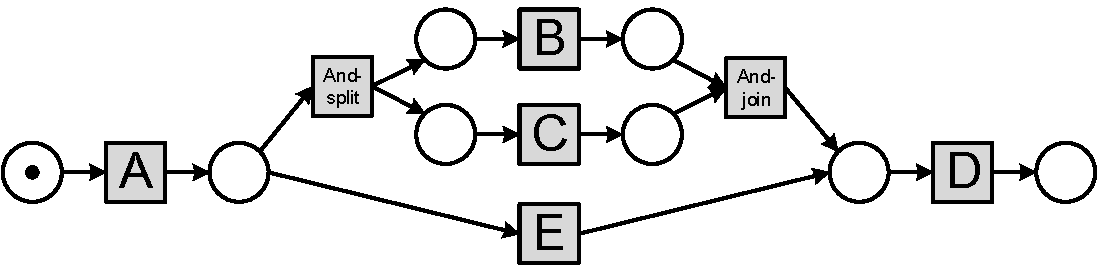
\includegraphics[width=1.0\textwidth]{petri_net_example}
  \caption{标识Petri网示例\label{fig:petri_net_example}}
\end{figure}

图\ref{fig:petri_net_example}展示了一个由8个库所和8个变迁组成的Petri网。变迁$A$有一个输入库所$p_{1}$和一个输出库所$p_{2}$,变迁$AND$-$split$有一个输入库所$p_{2}$和两个输出库所$p_{3}$、$p_{4}$,变迁$AND$-$join$有两个输入库所$p_{5}$、$p_{6}$和一个输出库所$p_{7}$。变迁$A$的输入库所中的黑点表示一个托肯(token),这个托肯即为该Petri网的初始标识。该Petri网的行为由如下发生规则定义。

\begin{definition}[发生规则]\label{def:firing_rule}
令$\Sigma=(N=(P,T,F),s)$是一个标识Petri网:
  \begin{itemize}
  	\item[-] 变迁$t\in T$被使能,记作$(N,s)[t\rangle$,当且仅当$\bullet t\leq s$;
  	\item[-] 发生规则$\_[\_\rangle\_\subseteq\mathcal{N}\times T\times\mathcal{N}$是满足如下条件的最小关系:\\$\forall (N=(P,T,F),s)\in\mathcal{N},\forall t\in T:(N,s)[t\rangle\Rightarrow(N,s)[t\rangle(N,s-\bullet t+t\bullet)$。
  \end{itemize}
\end{definition}

在图\ref{fig:petri_net_example}的标识Petri网(源库所有一个托肯)中,变迁$A$被使能。当变迁$A$发生后,会将其输入库所中的托肯移除,在其输出库所中加入一个托肯,如图\ref{fig:petri_net_example_fire1}所示。此时,变迁$E$和变迁$AND$-$split$都被使能。虽然两者都被使能,但是只有一个能够发生,因为变迁$E$和变迁$AND$-$split$此时会竞争唯一的托肯。如果变迁$AND$-$split$发生,会消耗其输入库所的托肯并在两个输出库所中各生成一个托肯,如图\ref{fig:petri_net_example_fire2}所示。

\begin{figure}[htbp]
  \centering
  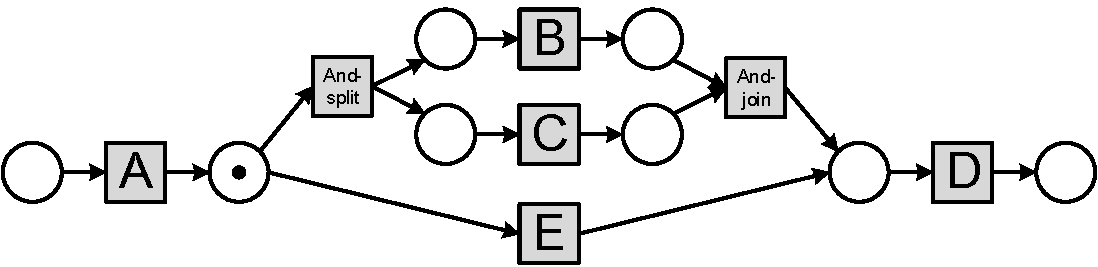
\includegraphics[width=1.0\textwidth]{petri_net_example_fire1}
  \caption{变迁$A$发生后的标识Petri网\label{fig:petri_net_example_fire1}}
\end{figure}

\begin{figure}[htbp]
  \centering
  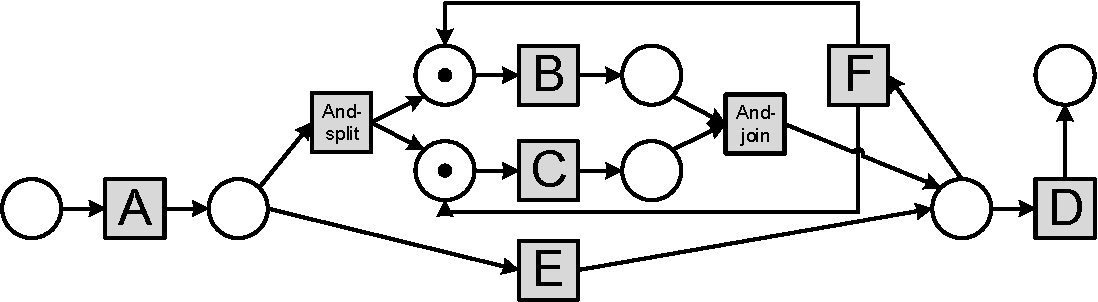
\includegraphics[width=1.0\textwidth]{petri_net_example_fire2}
  \caption{变迁$AND$-$split$发生后的标识Petri网\label{fig:petri_net_example_fire2}}
\end{figure}

\begin{definition}[可达标识]\label{def:reachable_markings}
令$(N,s_{0})\in\mathcal{N}$是一个标识Petri网。标识$s$从初始标识$s_{0}$可达,当且仅当存在一条变迁序列,其变迁依次发生使标识$s_{0}$变为$s$。$(N,s_{0})$所有可达标识的集合记作$[N,s_{0}\rangle$。
\end{definition}

图\ref{fig:petri_net_example}中的标识Petri网有八个可达标识。本文用如下方式描述到达某个可达标识的变迁发生序列。令$A$为标签集合。由$A$内元素组成的长度为$n\in\mathbb{N}$的序列是一个函数$\sigma:\{0,...,n-1\}\rightarrow A$。长度为0的序列称作空序列,记作$\varepsilon$。为了便于理解,一个长度大于0的序列通常简写为函数的值序列。例如,序列$\sigma=\{(0,a),(1,a),(2,b)\}$简写为$aab$。由$A$内元素组成的任意长度的所有序列集合记作$A^{*}$。

\begin{definition}[发生序列]\label{def:firing_sequence}
令$(N=(P,T,F),s_{0})$是一个标识Petri网。序列$\sigma\in T^{*}$是$(N,s_{0})$的一条发生序列当且仅当对于某个自然数$n\in\mathbb{N}$,存在标识$s_{1},...,s_{n}$和变迁$t_{1},...,t_{n}\in T$,使得$\sigma=t_{1}...t_{n}$,且对于所有满足$0\leq i\leq n$的$i$,$(N,s_{i})[t_{i+1}\rangle$且$s_{i+1}=s_{i}-\bullet t_{i+1}+t_{i+1}\bullet$。($n=0$隐含$\sigma=\varepsilon$,$\varepsilon$是$(N,s_{0})$的发生序列。)序列$\sigma$在标识$s_{0}$下可发生,记作$(N,s_{0})[\sigma\rangle$。序列$\sigma$发生后得到标识$s_{n}$,记作$(N,s_{0})[\sigma\rangle(N,s_{n})$。
\end{definition}

\begin{definition}[连通性]\label{def:connectedness}
网$N=(P,T,F)$是弱连通的,或者简称连通的,当且仅当对于任意两个节点$x,y\in P\cup T$,$x(F\cup F^{-1})y$,其中$R^{-1}$是关系$R$的逆,$R^{*}$是关系$R$的自反传递闭包。网$N$是强联通的,当且仅当对于任意两个节点$x,y\in P\cup T$,$xF^{*}y$。
\end{definition}

图\ref{fig:petri_net_example}中的标识Petri网是连通的,但不是强连通的,例如没有从汇库所到源库所的有向路径,也没有从变迁$D$到变迁$A$的有向路径。

\begin{definition}[有界性、安全性]\label{def:boundedness_safeness}
标识Petri网$(N=(P,T,F),s)$是有界的,当且仅当可达标识集合$[N,s\rangle$是有穷的。$(N,s)$是安全的,当且仅当$\forall s'\in[N,s\rangle,\forall p\in P,s.t.~s'(p)\leq 1$。显然,安全性隐含了有界性。
\end{definition}

图\ref{fig:petri_net_example}中的标识Petri网是安全的(也是有界的),因为它的八个可达标识中没有库所会包含超过一个托肯。

\begin{definition}[死变迁,活性]\label{def:dead_transition}
令$(N=(P,T,F),s)$是一个标识Petri网。变迁$t\in T$是死变迁当且仅当$\nexists s'\in[N,s\rangle,s.t.~(N,s')[t\rangle$。$(N,s)$是活的,当且仅当$\forall s'\in[N,s\rangle,\forall t\in T,s.t.~\exists s'\in[N,s'\rangle,(N,s')[t\rangle$。显然,活性隐含不存在死变迁。
\end{definition}

图\ref{fig:petri_net_example}中的标识Petri网的所有变迁都不是死变迁。但是它不是活的,因为它无法使每个变迁不断地发生。

\subsection{工作流网}\label{subsec:workflow_net}
大多数工作流系统提供了构建标准逻辑的连接语义词,例如$AND$-$split$,$AND$-$join$,$OR$-$split$和$OR$-$join$\cite{van2004workflowbook,fischer2002workflow,jablonski1996workflow,leymann2000production}。这些语义词被用于建模顺序、条件、并行和循环结构\cite{fischer2002workflow}。显然,Petri网拥有足够的能力来表达上述结构:用变迁表示任务,库所和边表示因果依赖。例如,库所可以表示任务的前驱条件或者后继条件;$AND$-$split$可以用含有多个输出库所的变迁表示;$OR$-$split$/$OR$-$join$可以用含有多条出边/入边的库所表示。

用于建模工作流中控制流维度的Petri网称作工作流网(Workflow net,缩写为WF-net)。工作流网最先由荷兰教授Wil M.P. van der Aalst提出\cite{van1998application}。

\begin{definition}[工作流网]\label{def:workflow_net}
令$N=(P,T,F)$是一个Petri网,$\overline{t}$是不属于$P\cup T$的新节点。$N$是工作流网(WF-net)当且仅当:
  \begin{itemize}
  	\item[-] 对象创建:$P$含有一个输入库所$i$满足:$\bullet i=\emptyset$;
  	\item[-] 对象完成:$P$含有一个输出库所$o$满足:$o\bullet=\emptyset$;
  	\item[-] 连通性:$\overline{N}=(P,T\cup\{\overline{t}\},F\cup\{(o,\overline{t}),(\overline{t},i)\})$是强连通的。
  \end{itemize}
\end{definition}

图\ref{fig:petri_net_example}中的标识Petri网是一个WF-net。虽然该网不是强连通的,但其短回路网$\overline{N}=(P,T\cup\{\overline{t}\},F\cup\{(o,\overline{t}),(\overline{t},i)\})$是强连通的。即使一个网满足定义\ref{def:workflow_net}中的所有条件,其对应的过程模型仍然可能包含诸如死锁、永远不被使能的任务、活锁、过程终止后有残留托肯等错误。因此,需要定义如下原则。

\begin{definition}[合理性]\label{def:sound}
令$N=(P,T,F)$为一个WF-net,其输入库所为$i$,输出库所为$o$。$N$是合理的,当且仅当:
  \begin{itemize}
  	\item[-] 安全性:$(N,[i])$是安全的;
  	\item[-] 恰当完成:$\forall s\in[N,[i]\rangle,s.t.~o\in s\Rightarrow s=[o]$;
  	\item[-] 可完成:$\forall s\in[N,[i]\rangle,s.t.~[o]\in[N,s\rangle$;
  	\item[-] 不含死任务:$(N,[i])$不包含死变迁。
  \end{itemize}
所有合理的WF-net组成集合$\mathcal{W}$。
\end{definition}

图\ref{fig:petri_net_example}中的WF-net是合理的。合理性可以用标准Petri网分析技术来验证。事实上,WF-net的合理性对应于其短回路网的活性和安全性\cite{van1997verification,van1998application,van2004workflowbook}。因此,可以应用高效的算法和工具验证WF-net的合理性,例如针对WF-net的裁剪分析工具Woflan\cite{verbeek2001diagnosing}。

\subsection{过程流}\label{subsec:process_run}
本文针对过程模型的任务间有序关系进行精炼,首先给出有序关系的标准定义。

\begin{definition}[任务间有序关系\cite{esparza2002improvement}]\label{def:ordering_relations}
Petri网的任意一对节点$x,y$之间有三种基本有序关系:
  \begin{itemize}
  	\item[-] $x$和$y$满足因果关系,当且仅当该网存在一条至少包含一条边、从$x$到$y$的路径,记作$x<y$;
  	\item[-] $x$和$y$满足冲突关系,当且仅当该网存在两条开始于同一个库所$s$的路径$st_{1}...x$和$st_{2}...y$,且$t_{1}...x$和$t_{2}...y$不相交,记作$x\#y$;
  	\item[-] $x$和$y$满足并行关系,当且仅当$x$和$y$既不满足因果关系,也不满足冲突关系,记作$x~co~y$。
  \end{itemize}
\end{definition}

如前文所述,本文对因果关系和并行关系进行精炼。为了便于定义与描述,本文使用过程流来描述仅含有上述两种关系的模型。使用过程流可以恰当地描述变迁发生序列中的因果和并行关系。一个网系统的过程流是一种称作因果网的特殊网,并使用一个函数将因果网的节点映射到原网系统的节点上。

\begin{definition}[因果网\cite{polyvyanyy20144c}]\label{def:causal_net}
$N=(B,E,G)$是因果网,当且仅当:
  \begin{itemize}
  	\item[-] 对于任意$b\in B$,满足:$|\bullet b|\leq 1$且$|b\bullet|\leq 1$;
  	\item[-] $N$是无环的,即$G^{+}$是非自反的。
  \end{itemize}
\end{definition}

$B$和$E$中的元素分别称为$N$的条件和事件。因果网$N=(B,E,G)$的两个节点$x$和$y$满足因果关系,当且仅当$(x,y)\in G^{+}$;$x$和$y$满足并行关系,当且仅当$x\neq y$,$(x,y)\notin G^{+}$且$(y,x)\notin G^{+}$。一个因果网的割是其所有俩俩并行条件的最大集合。

因果网的事件可以用来描述变迁发生序列。

\begin{definition}[过程流\cite{polyvyanyy20144c}]\label{def:process_run}
标识Petri网$(N=(P,T,F),s)$的过程流是一个有序二元组$\pi=(N_{\pi},\rho)$,其中$N_{\pi}=(B,E,G)$是一个因果网,$\rho:B\cup E\rightarrow P\cup T$是一个映射函数且满足如下条件:
  \begin{itemize}
  	\item[-] $\rho(B)\subseteq P$且$\rho(E)\subseteq T$;
  	\item[-] $Min(N_{\pi})$是一个割且$\forall p\in P:s(p)=|\rho^{-1}(p)\cap Min(N_{\pi})|$,即$\pi$的初始标识是$s$;
  	\item[-] 对于任意事件$e\in E$和任意库所$p\in P$满足:$\bm{1}_{F}((p,\rho(e)))=|\rho^{-1}(p)\cap\bullet e|$且$\bm{1}_{F}((\rho(e),p))=|\rho^{-1}(p)\cap e\bullet|$.\footnote{$\bm{1}_{F}$表示$F$在集合$(P\times T)\cup(T\times P)$上的特征函数。}
  \end{itemize}
\end{definition}

给定一个过程流$\pi$,事件集合$E$和映射函数$\rho$经常被记作$E_{\pi}$和$\rho_{\pi}$。一个标识Petri网$S$所有过程流的集合记作$\Pi_{S}$。前文提到的因果关系和并行关系同样可以定义在$\pi$的因果网节点上,分别记作$\rightarrowtail_{\pi}$和$\parallel{\pi}$,在含义明确的情况下脚标常被省略。

\begin{figure}[htbp]
  \centering
  \begin{subfigure}{1\textwidth}
  	\centering
  	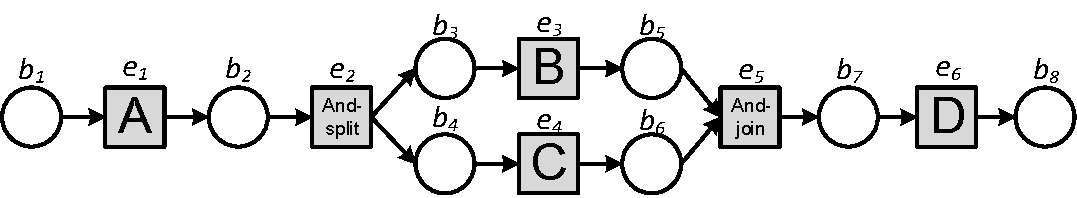
\includegraphics[width=0.65\textwidth]{process_run_example_1}
  	\caption{\label{fig:process_run_example_1}}
  \end{subfigure}
  \begin{subfigure}{1\textwidth}
  	\vspace{1em}
  	\centering
  	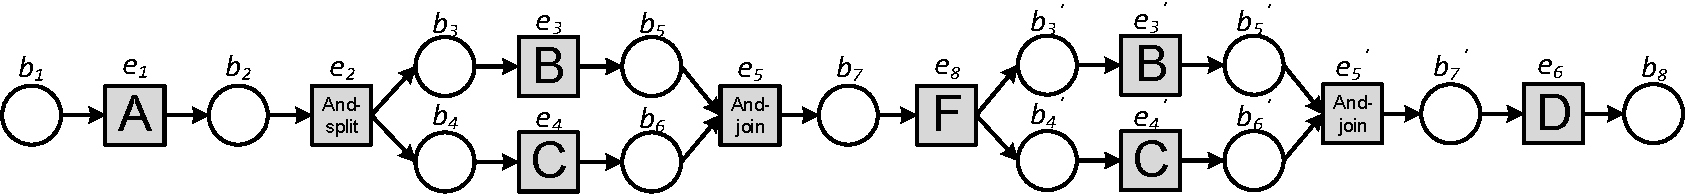
\includegraphics[width=1\textwidth]{process_run_example_2}
  	\caption{\label{fig:process_run_example_2}}
  \end{subfigure}
  \vspace{6pt}
  \caption{图\ref{fig:petri_net_example}中模型的两个过程流示例}
\end{figure}

图\ref{fig:process_run_example_1}和图\ref{fig:process_run_example_2}展示了图\ref{fig:petri_net_example}中模型的两个过程流$\pi_{1}$和$\pi_{2}$。当对过程流进行图形化展示时,条件$c_{i},c_{i}'...$对应于库所$p_{i}$,即$\rho(c_{i})=\rho(c_{i}')=p_{i}$。类似的,事件$e_{j},e_{j}'...$对应于变迁$t_{j}$,即$\rho(e_{j})=\rho(e_{j}')=t_{j}$。在图\ref{fig:process_run_example_2}中,$e_{3}\parallel e_{4}$、$e_{4}\rightarrow e_{4}'$、$e_{3}'\parallel e_{4}'$。显然,若两个事件在一个Petri网$N$的过程流$\pi$中满足因果关系,则它们在原网中对应的变迁必然能在某个变迁发生序列中顺序发生。类似的,若两个事件在$\pi$中满足并行关系,则它们在原网中对应的变迁必然会在某个可达标识$s$下同时被使能,而且可以在$s$这个标识下以任意顺序发生。

每个事件$e\in E_{\pi}$都代表着对应变迁$\rho_{\pi}(e)$的一次发生。J{\"o}rg Desel等人给出了一个网系统的过程流与其变迁发生序列对应的方法\cite{desel2000validation}。给定一个Petri网,对其过程流加标识得到$(N_{\pi},s)$,其中$N_{\pi}$是该网过程流$(N_{\pi},\rho)$的因果网且标识$s$仅在每个源条件中放置一个托肯。通过映射函数$\rho$可以将该过程流的事件发生序列与原网的变迁发生序列对应起来。例如,图\ref{fig:process_run_example_1}中的过程流的事件发生序列可以对应图\ref{fig:petri_net_example}中模型的变迁发生序列$t_{1}t_{2}t_{3}t_{4}t_{5}t_{6}$。

\subsection{完全前缀展开}\label{subsec:cpu}
在一个模型的所有过程流中,只有因果关系和并行关系被抽取出来。因此,在一个过程流中只存在顺序和并发结构,而不存在循环和互斥结构。然而,由于过程模型中循环结构的存在,一个模型可能有无穷多个过程流,区别在于循环结构展开的程度。显然,使用这无穷多个过程流去抽取ExRORU是不现实的。Javier Esparza等人提出了完全前缀展开(Complete Prefix Unfolding,简称CPU)的概念来避免此问题\cite{esparza2002improvement}。

考虑一个含有根节点的有向图$G$。众所周知该图可以被展开成一棵带有标签的树(树的节点正好是图$G$中从根节点开始的所有路径上的点)。树上的节点标签由图中的节点决定。上述展开过程可以在任意时间停止,从而得到不同的树。显然,如果尽可能多地将图展开,总会得到一棵唯一的标签树,通常是无穷大的。这棵最大的树称为该图的展开(unfolding)。

类似的,Petri网也可以被展开成带标签的发生网(occurrence nets,是一种带有类树型结构的简单图)。发生网的节点标签由原网的库所和标签决定。通过一个Petri网展开得到的发生网被称作分支过程(branching processes)。展开过程可以在任意时间停止,从而得到不同的分支过程。显然,如果尽可能多地将Petri网展开,总会得到一个唯一的分支过程,通常是无穷大的。这个最大的分支过程称为该Petri网的展开。

\begin{definition}[发生网]\label{def:occurrence_net}
发生网$O=(B,E,F)$是满足如下条件的网:
  \begin{enumerate}[(1)]
  	\item $\forall b\in B,|\bullet b|\leq 1$;
  	\item $O$是无环网,或者说该网的因果关系是一种偏序关系;
  	\item $O$是有穷前驱的,即,对于任意节点$x\in B\cup E$,满足$y<x$的元素$y\in B\cup E$的集合是有穷的;
  	\item 没有元素与自身冲突。
  \end{enumerate}
\end{definition}

显然,发生网中的任意两个节点间正好满足定义\ref{def:ordering_relations}中的三种关系之一。$B$和$E$中的元素通常被称为条件和事件。$Min(O)$表示$B\cup E$中前集为空的元素集合。由于在合理WF-net中所有的变迁前集都不为空,所以$Min(O)$中的元素只有条件。

\begin{definition}[分支过程]\label{def:branching_process}
标识Petri网$\Sigma=(P,T,F,s_{0})$的分支过程是一个标签发生网$\beta=(O,p)=(B,E,F,p)$,其中函数$p$满足如下性质:
  \begin{enumerate}[(i)]
  	\item $p(B)\subseteq P$且$p(E)\subseteq T$($p$保持了节点的本性);
  	\item 对于任意$e\in E$,函数$p$对于$\bullet e$的约束是一个从$\bullet e$($\sigma$中)到$\bullet p(e)$($\beta$中)的双射,$e\bullet$和$p(e)\bullet$类似($p$保持了标签的环境);
  	\item 函数$p$对$Min(O)$的约束是一个从$Min(O)$到$s_{0}$的双射($\beta$从$s_{0}$“开始”);
  	\item $\forall e_{1},e_{2}\in E:\bullet e_{1}=\bullet e_{2}\wedge p(e_{1})=p(e_{2})\Rightarrow e_{1}=e_{2}$($\beta$不会重复$\Sigma$中的变迁)。
  \end{enumerate}
\end{definition}

\begin{figure}[htbp]
  \centering
  \begin{subfigure}{1\textwidth}
  	\centering
  	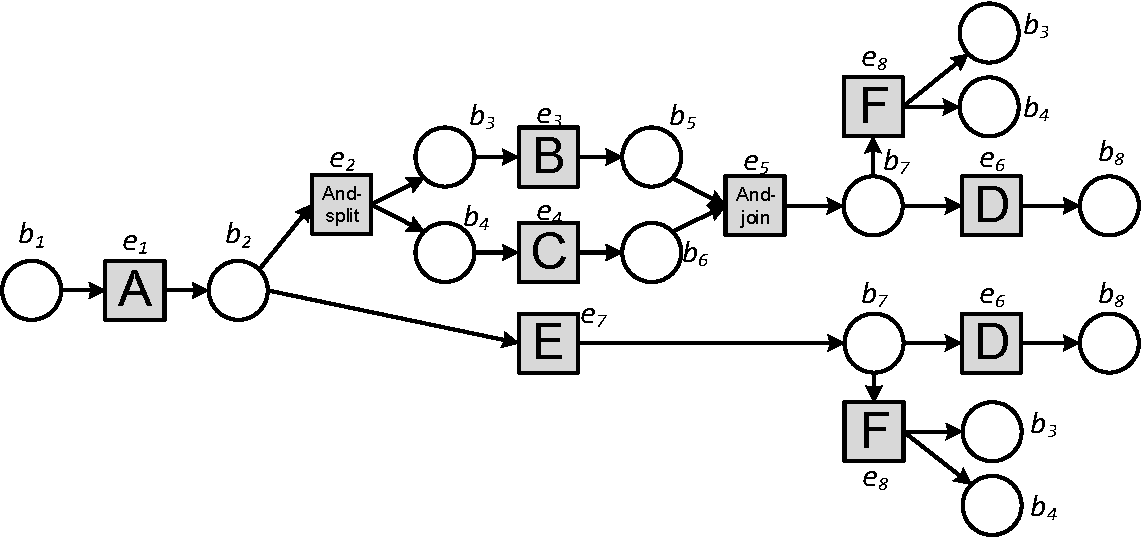
\includegraphics[width=0.7\textwidth]{branching_process_example_1}
  	\caption{\label{fig:branching_process_example_1}}
  \end{subfigure}
  \begin{subfigure}{1\textwidth}
  	\vspace{1em}
  	\centering
  	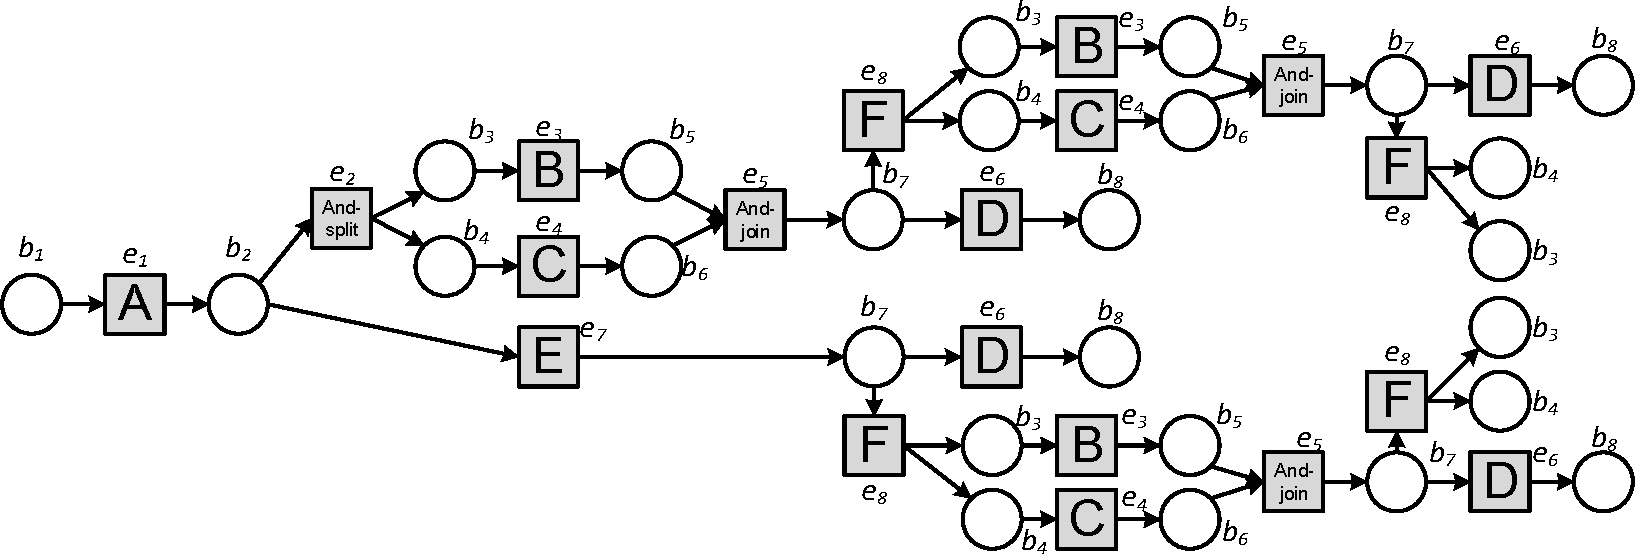
\includegraphics[width=1\textwidth]{branching_process_example_2}
  	\caption{\label{fig:branching_process_example_2}}
  \end{subfigure}
  \vspace{6pt}
  \caption{图\ref{fig:petri_net_example}中模型的两个分支过程}
  \label{fig:branching_process_example}
\end{figure}

图\ref{fig:branching_process_example_1}和图\ref{fig:branching_process_example_2}展示了图\ref{fig:petri_net_example}中模型的两个分支过程。分支过程的差别在于它们展开的程度,展开少的分支过程是那些展开的多的分支过程的前缀。

\begin{definition}[分支过程前缀]\label{def:branching_process_prefix}
令$\beta'=(O',p')$和$\beta=(O,p)$是一个标识Petri网的两个分支过程。$\beta'$是$\beta$的前缀,当且仅当$O'$是$O$的子图且满足如下条件:
  \begin{itemize}
  	\item[-] $Min(O)$属于$O'$;
  	\item[-] 如果条件$b$属于$O'$,那么它在$O$中的输入事件$e\in\bullet b$也属于$O'$(如果存在的话);
  	\item[-] 如果事件$e$属于$O'$,那么它在$O$中的输入和输出条件$\bullet e\cup e\bullet$也属于$O'$。
  \end{itemize}
  $p'$是函数$p$在$O'$上的对应。
\end{definition}

根据上述前缀定义,一个Petri网总有一个唯一的最大分支过程\cite{engelfriet1991branching},即前文所述的Petri网展开。图\ref{fig:petri_net_example}中模型的展开是无穷大的。

一个分支过程有一个自然的初始标识,即在每个源条件内放置一个托肯。据此,可以形式化一个展开如何描述Petri网的行为:令$\Sigma$是一个标识Petri网,$\beta$是它的展开。$\Sigma$和$\beta$的可达图有着同构化的展开形式。$\Sigma$的可达标识就是满足$s$是$\beta$的可达标识的那些$p(s)$;对于$\beta$的一个可达标识$s$和$\Sigma$的可达标识$s''$、变迁$t$,存在可达标识$s'$和事件$e$满足$p(s')=s''$,$p(e)=t$且$s\overset{e}{\rightarrow}s'$当且仅当在$\Sigma$中$p(s)\overset{t}{\rightarrow}s''$成立。

\begin{definition}[完全前缀展开,CPU]\label{def:cpu}
令$O=(B,E,A,p)$是一个发生网,其中$p$是发生网节点到原始标识Petri网节点的多对一映射,$e\in E$是任意事件。
  \begin{itemize}
  	\item[-] 事件$e$的局部配置$\lceil e\rceil$是在$e$之前可达$e$的事件集合;
  	\item[-] 局部配置$\lceil e\rceil$的终结标识$Mark(\lceil e\rceil)$是在$\lceil e\rceil$中事件都被触发后被标识的事件集合;
  	\item[-] 充分顺序$\prec$是定义在局部配置上的严格有根据的偏序关系,满足$\lceil e\rceil\subset\lceil e'\rceil\Rightarrow\lceil e\rceil\prec\lceil e'\rceil\Rightarrow$\footnote{这里使用了\onlinecite{esparza2002improvement}中在1-安全Petri网上定义的完全顺序关系。};
  	\item[-] 事件$e$被称为截断事件,当且仅当存在一个关联事件$e'$满足$Mark(\lceil e\rceil)=Mark(\lceil e'\rceil)$且$\lceil e'\rceil\prec\lceil e\rceil$;
  	\item[-] 完全前缀展开是一个发生网的最大后向闭包子图,且在截断事件后没有任何事件。
  \end{itemize}
\end{definition}

\begin{figure}[htbp]
  \centering
  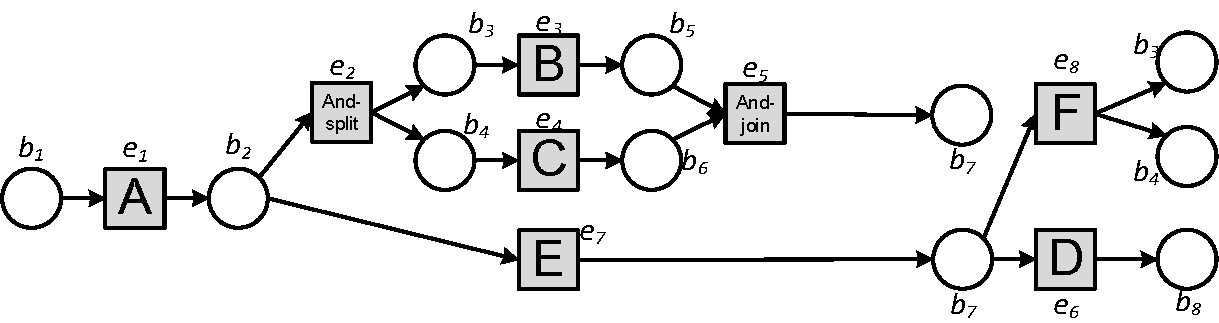
\includegraphics[width=1\textwidth]{cpu_example}
  \caption{图\ref{fig:petri_net_example}中模型的CPU\label{fig:cpu_example}}
\end{figure}

图\ref{fig:cpu_example}展示了图\ref{fig:petri_net_example}中模型的CPU。在该CPU中,事件$AND$-$join$和事件$F$是截断事件。事件$AND$-$join$的关联事件是$E$,$F$的关联事件是$AND$-$split$。

显然,将一个模型的CPU从截断事件后面继续展开可以得到这个模型的所有过程流。换句话说,CPU是一个模型最小但最完整的过程流表达。因此,本文使用过程流来定义所有的关系,并使用CPU来高效计算它们。

\section{当前面临的挑战}\label{sec:challenge}
本文主要工作在于对RORU算法的扩展上,因此有必要探讨原算法所面临的挑战。本文之所以选择RORU作为研究基础,一方面是因为它是定义在被广泛使用的WF-net上,有很多成熟的建模和分析工具可以利用,且其算法能被扩展到使用各种语言建模的过程模型中;另一方面,RORU对过程行为语义进行了细致的刻画,且给出了高效、准确的计算方法。本小节只简单列举RORU的部分不足之处,更详细的讨论会在本文后续章节中涉及。本文提出的ExRORU同样定义在WF-net上,但是与RORU相似,其思路可以被扩展到使用各种语言建模的过程模型中。

{\heiti 循环结构。}正如\onlinecite{jin2014computing}所述,RORU算法针对无环过程模型。然而实际生活中,大约10\%-20\%都是含有循环结构的。所以RORU对于环处理的缺失会大大降低其能力。

{\heiti 不可见任务。}不可见任务是指过程模型中存在,但是实际执行日志中并不存在的任务。RORU将不可见任务也作为普通可见任务处理,然而过程模型中可能存在充当路由功能的无意义任务。另外,在变迁发生序列中信息的缺失和噪声的存在都可能导致挖掘过程产生不可见任务。目前,RORU并没有考虑不可见任务对过程模型行为的影响,所以无法正确处理含有不可见任务的模型。

{\heiti 非自由选择结构。}为了还原过程模型两个变迁之间的关系,需要将其CPU中对应事件的关系进行映射。在含有非自由选择结构的过程模型的CPU中会出现重名事件,导致事件间的关系不唯一。RORU并未考虑重名事件的影响。

{\heiti 紧邻关系。}上述两种结构的存在会使得一些结构上并不紧邻的事件在事件发生序列中紧邻发生,从而影响其行为语义。RORU未考虑事件间紧邻关系的存在,故对一些行为相似但不一致的模型无法区分。

本文重点对以上不足之处进行改进,探讨如何应对这些挑战。

\section{论文的主要贡献}\label{sec:contribution}
本文尝试对RORU算法\cite{jin2014computing}的不足进行扩展,主要有以下几点贡献:
\begin{enumerate}[1.]
  \item 提出了扩展不确定性精炼任务间关系,即ExRORU。利用ExRORU可以刻画所有类型的合理过程模型,包括含有循环结构、不可见任务及非自由选择结构的模型。
  \item 探讨ExRORU如何能识别任意一堆过程模型之间的行为差异,即给出一个过程模型行为语义的唯一刻画。
  \item 给出ExRORU算法的实现并在效率、能力和可扩展性上将其与现有的计算任务间关系的主流算法进行比较。
\end{enumerate}

\section{论文章节安排}\label{sec:structure}
本文章节安排如下,第\ref{cha:intro}章对全文进行概述,介绍本文选题背景和意义、涉及到的基本知识以及当前算法所面临的主要挑战,从而引出本文的工作重点。第\ref{cha:related_work}章主要介绍过程模型行为刻画方法的研究现状,分类介绍了国内外学者提出的各类算法并分析其优缺点,尤其重点介绍了本文基础RORU算法的处理能力和不足之处。第\ref{cha:exroru}章详细阐述了ExRORU的定义和计算方法,并探讨了其检测任意一对过程模型行为差异的能力,并重点分析了事件间ExRORU和变迁间ExRORU关系的相互关系。第\ref{cha:experiment}章给出了ExRORU算法的实现并将其与现有的计算任务间关系的主流算法进行了比较,此外还重点将其与RORU进行了效率、能力等方面的对比。第\ref{cha:conclusion}章对本文工作进行总结并对未来工作进行了展望。